% ============================================================
%  DiffuVQA — Graduation Poster
%  CENG416 — A0 Vertical (841mm x 1189mm)
%  Overleaf: compile with XeLaTeX or pdfLaTeX
% ============================================================
\documentclass[final]{beamer}

\usepackage[
  orientation=portrait,
  size=a0,
  scale=1.3          % base font scale; title/heading sizes set below
]{beamerposter}

\usepackage[utf8]{inputenc}
\usepackage[T1]{fontenc}
\usepackage{lmodern}
\usepackage{graphicx}
\usepackage{booktabs}
\usepackage{multirow}
\usepackage{amsmath,amssymb}
\usepackage{tikz}
\usetikzlibrary{arrows.meta, positioning, shapes.geometric, calc}
\usepackage{xcolor}
\usepackage{setspace}
\usepackage{ragged2e}   % \justifying

% ── Colour palette ──────────────────────────────────────────
\definecolor{headerblue}{RGB}{163,31,52}
\definecolor{accentred}{RGB}{120,15,30}
\definecolor{lightgray}{RGB}{245,245,245}
\definecolor{darkgray}{RGB}{60,60,60}
\definecolor{sectionbg}{RGB}{245,220,225}

% ── Beamer theme ────────────────────────────────────────────
\usetheme{default}
\setbeamercolor{background canvas}{bg=white}
\setbeamercolor{block title}{fg=white, bg=headerblue}
\setbeamercolor{block body}{fg=darkgray, bg=lightgray}
\setbeamerfont{block title}{size=\large, series=\bfseries}
\setbeamerfont{block body}{size=\normalsize}
\setbeamertemplate{navigation symbols}{}
\setbeamertemplate{caption}[numbered]

\setbeamerfont{title}{size=\Huge, series=\bfseries}
\setbeamerfont{author}{size=\Large}
\setbeamerfont{institute}{size=\large}

\newcommand{\postersection}[2]{%
  \begin{block}{\LARGE #1}
    \justifying\large #2
  \end{block}
}

% ============================================================
\begin{document}
\begin{frame}[t, fragile]

% ── HEADER ──────────────────────────────────────────────────
\begin{columns}[t]
  \begin{column}{0.15\linewidth}
    \vspace{1cm}
    \begin{center}
      
\includegraphics[width=0.85\linewidth]{iyte_logo.png}
    \end{center}
  \end{column}

  \begin{column}{0.70\linewidth}
    \vspace{0.5cm}
    \begin{center}
      {\Huge\bfseries\color{headerblue}
        DiffGenMed-VQA: Diffusion-Based Generative\\[0.3ex]
        Medical Visual Question Answering
      }\\[0.8em]
      {\Large\color{darkgray}
        Ali Ekin Özçetin\textsuperscript{1}\quad
        Ahmet Barış Özel\textsuperscript{2}\quad
        Mert Güner\textsuperscript{3}
      }\\[0.3em]
      {\large\color{darkgray}
        Advisor: Prof.\ Dr.\ Aytuğ Onan
      }\\[0.4em]
      {\large\color{darkgray}
        Department of Computer Engineering,
        İzmir Institute of Technology (IYTE)
      }\\[0.3em]
      {\normalsize\color{darkgray}
        \textbf{Code:} \texttt{github.com/Aliekinozcetin/DiffuVQA-Original}
        \quad
      }
    \end{center}
  \end{column}

  \begin{column}{0.15\linewidth}
    \vspace{1cm}
    \begin{center}
      
\includegraphics[width=0.85\linewidth]{iyte_logo.png}
    \end{center}
  \end{column}
\end{columns}

\vspace{0.1cm}
\noindent\textcolor{headerblue}{\rule{\linewidth}{3pt}}

% ── THREE-COLUMN BODY ────────────────────────────────────────
\begin{columns}[t]

% ════════════════════════════════
%  COLUMN 1
% ════════════════════════════════
\begin{column}{0.31\linewidth}

  % ── Abstract / Summary ──────────────────────────────────
  \postersection{Abstract}{%
    Medical Visual Question Answering (Med-VQA) aims to generate accurate
    answers to clinical questions about medical images. While existing
    approaches rely on \textbf{classification over fixed answer sets}, we
    propose \textbf{DiffGenMed-VQA}, a generative framework that produces
    free-form answers through \textbf{conditional diffusion over continuous
    embedding space}. Our system integrates a \textbf{CLIP vision encoder}
    with biomedical language encoders via cross-modal feature fusion,
    conditioned through \textbf{CIGN} (Conditional Information Gaussian
    Noising) --- a bidirectional mechanism that injects multimodal context
    into both forward and reverse diffusion.
  }

  \vspace{0.2cm}

  % ── Background / Literature Review ──────────────────────
  \postersection{Background \& Related Work}{%
    Conventional Med-VQA frames answer generation as \textbf{classification over fixed vocabularies}, limiting clinical expressivity. Recent \textbf{continuous diffusion} approaches enable iterative, globally coherent text generation beyond autoregressive constraints.

    \vspace{0.8em}

    \begin{center}
    \begin{tikzpicture}[
      node distance=0cm,
      every node/.style={font=\large},
      box/.style={
        rectangle, rounded corners=5pt,
        draw=headerblue, fill=sectionbg,
        text width=0.88\linewidth, align=left,
        inner sep=8pt, minimum height=1.6cm
      },
      ours/.style={
        box, draw=accentred, fill=accentred!12,
        font=\large\bfseries
      },
      arr/.style={-{Stealth[length=8pt]}, line width=1.5pt, color=headerblue}
    ]
      \node[box] (dlm) {
        \textbf{Diffusion-LM} \hfill \small NeurIPS '22\\
        \large Pioneered continuous embedding denoising for controllable text generation, enabling iterative refinement over dense word vectors.
      };
      \node[box, below=0.45cm of dlm] (ds) {
        \textbf{DiffuSeq} \hfill \small ICLR '23\\
        \large Extended diffusion to sequence-to-sequence tasks with partial noising, conditioning the reverse process on source text embeddings.
      };
      \node[box, below=0.45cm of ds] (sds) {
        \textbf{SeqDiffuSeq} \hfill \small NAACL '24\\
        \large Introduced self-conditioning and encoder-decoder separation, improving stability for short structured sequence outputs.
      };
      \node[ours, below=0.45cm of sds] (ours) {
        \textbf{DiffGenMed-VQA} \hfill \color{accentred}\small Ours, 2026\\
        \large First diffusion LM applied to medical VQA with CIGN bidirectional conditioning and systematic encoder comparison on clinical data.
      };
      \draw[arr] (dlm.south) -- (ds.north);
      \draw[arr] (ds.south)  -- (sds.north);
      \draw[arr] (sds.south) -- (ours.north);
    \end{tikzpicture}
    \end{center}


  }

  \vspace{0.3cm}

  % ── UN SDG Alignment ────────────────────────────────────────
  \postersection{UN SDG Alignment}{%
    \begin{tabular}{@{} p{0.16\linewidth} p{0.59\linewidth} p{0.15\linewidth} @{}}
      \toprule
      \textbf{SDG} & \textbf{Goal} & \textbf{Impact} \\
      \midrule
      \textbf{3}       & Good Health \& Well-being    & Direct   \\[0.3em]
      \textbf{8}       & Decent Work \& Econ.\ Growth & Direct   \\[0.3em]
      \textbf{10}      & Reduced Inequalities         & Indirect \\[0.3em]
      \textbf{16}      & Peace, Justice \& Inst.      & Indirect \\[0.3em]
      \textbf{11--13}  & Sustainable Development      & Indirect \\
      \bottomrule
    \end{tabular}
  }

\end{column}
\hfill

% ════════════════════════════════
%  COLUMN 2 (Method, Dataset ve Results)
% ════════════════════════════════
\begin{column}{0.35\linewidth}

  % ── Architecture & Methodology ──────────────────────────
  \postersection{Method \& Architecture}{%
    
    % Research Question Entegrasyonu
    \begin{center}
      \colorbox{sectionbg}{\parbox{0.96\linewidth}{\centering\normalsize\bfseries\itshape
        Can a diffusion-based generative model produce accurate free-form 
        answers to medical visual questions?
      }}
    \end{center}
    
    \vspace{0.4em}
    \begin{center}
    \begin{tikzpicture}[
      block/.style={
        rectangle, draw=headerblue, fill=lightgray,
        rounded corners=4pt, text width=0.38\linewidth, align=center,
        font=\small\bfseries, inner sep=8pt, minimum height=1.6cm
      },
      fusion/.style={
        rectangle, draw=headerblue, fill=sectionbg,
        rounded corners=4pt, text width=0.72\linewidth, align=center,
        font=\small\bfseries, inner sep=8pt, minimum height=1.4cm
      },
      diff/.style={
        rectangle, draw=accentred, fill=accentred!10,
        rounded corners=4pt, text width=0.92\linewidth, align=center,
        font=\small\bfseries, inner sep=10pt, minimum height=1.8cm
      },
      arrow/.style={-{Stealth[length=9pt]}, line width=1.6pt, color=headerblue}
    ]
      % --- Row 1: Two separate encoder boxes, side by side ---
      \node[block] (vision) {Vision Encoder\\[2pt]\mdseries\small CLIP ViT-B/32};
      \node[block, right=0.6cm of vision] (lang)
        {Language Encoder\\[2pt]\mdseries\small BERT / BioBERT / PubMedBERT};
      % --- Row 2: Fusion, centered below the two encoders ---
      \node[fusion, below=1.8cm of $(vision.south)!0.5!(lang.south)$, anchor=north] (fuse)
        {Cross-Modal Fusion \quad $(\alpha,\beta,\theta)$ dynamic weighting};
      % --- Row 3: Diffusion core ---
      \node[diff, below=1cm of fuse] (cign)
        {Diffusion Language Model via CIGN\\[3pt]
         \mdseries\small Denoises target answer embeddings conditioned on multimodal features $(q, v)$};
      % --- Arrows: each encoder drops straight down into fusion's top edge ---
      \draw[arrow] (vision.south) -- (vision.south |- fuse.north);
      \draw[arrow] (lang.south)   -- (lang.south   |- fuse.north);
      \draw[arrow] (fuse.south)   -- (cign.north);
    \end{tikzpicture}
    \end{center}

    \vspace{0.4em}
    {\large\textbf{Key Hyperparameters:}}
    \vspace{0.3em}
    \begin{center}
    \large
    \begin{tabular}{llll}
      \toprule
      $T{=}2{,}000$ & $d{=}768$ & heads${=}8$ & $L{=}32$ \\
      lr${=}1\text{e-}5$ & steps${=}150$k & noise$=$sqrt & DDIM${=}200$ \\
      \bottomrule
    \end{tabular}
    \end{center}
    
    \vspace{0.4em}
    \textbf{DiffGenMed-VQA} maps clinical question--image pairs into a continuous embedding space, bypassing classification limits via three stages: a \textbf{CLIP ViT-B/32} extracts visual features while a biomedical BERT variant encodes the question; a \textbf{Cross-Modal Fusion} block aligns both streams through dynamically weighted $(\alpha,\beta,\theta)$ attention; finally, the \textbf{CIGN-conditioned diffusion} core iteratively denoises target answer embeddings under the joint multimodal condition $(q, v)$ to produce free-form clinical answers.
  }
  
  % ── Dataset — Kvasir-VQA ────────────────────────────────
\postersection{Dataset — Kvasir-VQA}{%
  \begin{center}
  \large
  \renewcommand{\arraystretch}{0.8}
  \begin{tabular}{lrr}
    \toprule
    \textbf{Split} & \textbf{\# Questions} & \textbf{\# Images} \\
    \midrule
    Train & 47,079 & 5,200 \\
    Valid &  5,884 &   650 \\
    Test  &  5,886 &   650 \\
    \bottomrule
  \end{tabular}
  \end{center}

  \vspace{0.2em}
  \large
  Domain: gastrointestinal endoscopy. Target answer token length is tightly bounded ($\approx$2.9 tokens mean), restricting continuous rounding search fields.
}

  \vspace{0.5cm}

  % ── Results ─────────────────────────────────────────────
  \postersection{Results}{%

    \large
    \textbf{Quantitative Evaluation on Kvasir-VQA Test Set:}

    \vspace{0.4em}
    \begin{table}
      \begin{center}
      \large
      \renewcommand{\arraystretch}{0.8}
      \begin{tabular}{lccccc}
        \toprule
        \textbf{Encoder} & \textbf{EM} & \textbf{F1} & \textbf{BL-1} & \textbf{Y/N} & \textbf{Open} \\
        & \textbf{(\%)} & \textbf{(\%)} & & \textbf{(\%)} & \textbf{(\%)} \\
        \midrule
        \textbf{BERT-Base}  & 7.1  & 8.3  & 0.087  & 8.7   & 1.75 \\
        \textbf{BioBERT}    & 8.1  & 9.6  & 0.0723 & 12.95 & 3.5  \\
        \textbf{PubMedBERT} & 10.2 & 19.8 & 0.158  & 19.6  & 2.55 \\
        \bottomrule
      \end{tabular}
      \end{center}
      \caption{Quantitative baseline performance comparison metrics under strict leak-free protocol.}
    \end{table}

    \vspace{0.5em}

    \begin{center}
      \begin{figure}
        \includegraphics[width=\linewidth]{03_nlg_metrics_bar.png}
        \caption{NLG and semantic baseline metric yields ($n=1$).}
      \end{figure}
    \end{center}

    
  }
  
\end{column}
\hfill

% ════════════════════════════════
%  COLUMN 3
% ════════════════════════════════
\begin{column}{0.31\linewidth}

  % ── Loss Curve ──
  \begin{center}
    \begin{figure}
      \includegraphics[width=\linewidth]{01_loss_curve.jpeg}
      \caption{Continuous diffusion training loss curve across 150k steps.}
    \end{figure}
  \end{center}


  % ── Qualitative Examples ────────────────────────────────
  \postersection{Qualitative Examples}{%
    \begin{center}
    \normalsize
    \begin{tabular}{p{0.42\linewidth} | p{0.26\linewidth} | p{0.26\linewidth}}
      \toprule
      \textbf{Question} & \textbf{Reference} & \textbf{Generated} \\
      \midrule
      does this image contain any finding? & no & no \\
      \addlinespace[0.1em]
      are there any anatomical landmarks in the image? & none & none \\
      \addlinespace[0.1em]
      where in the image is the abnormality? & center; center-left; center-right & none \\
      \bottomrule
    \end{tabular}
    \end{center}

    \vspace{0.1em}
    \begin{center}
      \begin{figure}
        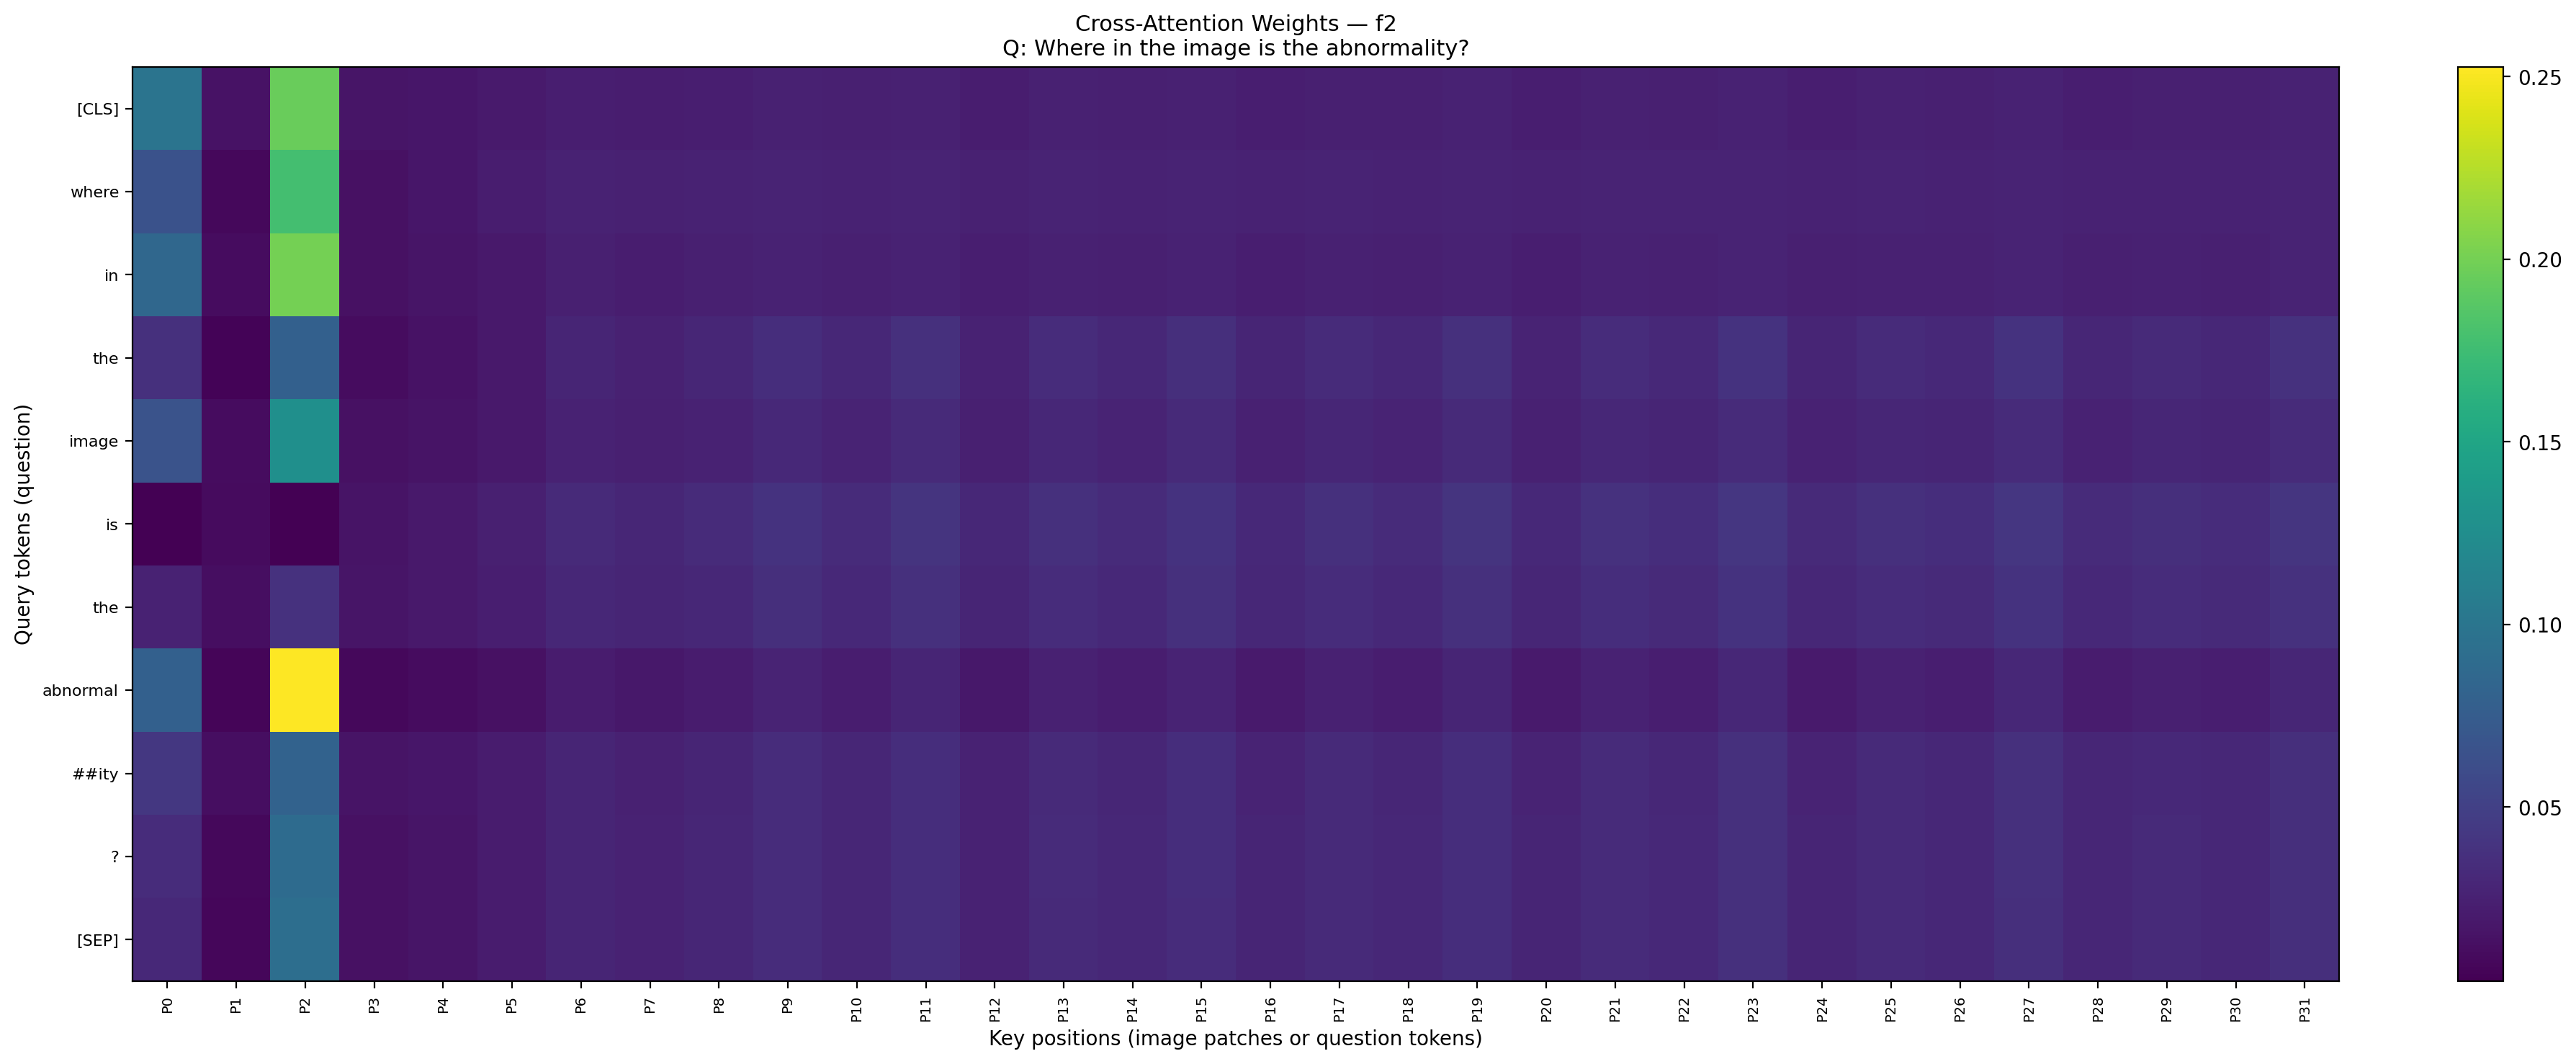
\includegraphics[width=0.98\linewidth]{cross_attention_heatmap.png}
        \caption{Cross-attention weights showing visual-textual alignment for the query \textit{``Where in the image is the abnormality?''}}
      \end{figure}
    \end{center}
  }


  % ── Conclusion ──────────────────────────────────────────
  \postersection{Conclusion \& Future Work}{%
    \textbf{Core Findings:}
    \begin{itemize}\large
      \item Generative continuous diffusion for Med-VQA is highly feasible but demands tighter constraints than token classification.
      \item Systematic evaluation reveals that domain-specific language encoders (\textbf{PubMedBERT}) provide more cohesive structural geometry under Gaussian noise.
      \item Our sampling-time clamping optimization effectively counteracts embedding collapse without additional retraining cycles.
    \end{itemize}

    \vspace{0.1em}
    \textbf{Future Work:}
    \begin{itemize}\large
      \item Implementing self-conditioning mechanics (\textit{SeqDiffuSeq}) to stabilize short med-answers.
      \item Incorporating token-level adaptive noise distributions to balance short sequence outputs.
    \end{itemize}
  }

  \vspace{0.1cm}

  % ── References ──────────────────────────────────────────
  \postersection{References}{%
    {\normalsize
    \begin{enumerate}
      \item Li et al. \textit{Diffusion-LM.} NeurIPS 2022.
      \item Gong et al. \textit{DiffuSeq.} ICLR 2023.
      \item Liu et al. \textit{DiffuVQA: Conditional Generative Diffusion for VQA.} Biomed.\ Signal Process.\ Control, 2026.
      \item Devlin et al. \textit{BERT.} NAACL-HLT 2019.
      \item Lee et al. \textit{BioBERT.} Bioinformatics, 2020.
      \item Gu et al. \textit{PubMedBERT.} ACM Trans.\ Comput.\ Healthcare, 2021.
      \item Radford et al. \textit{CLIP.} ICML 2021.
    \end{enumerate}
    }
  }

\end{column}
\end{columns}


\end{frame}
\end{document}